%built list of things I did
\documentclass{article}

\usepackage{graphicx}
\graphicspath{ {.} }
\DeclareGraphicsExtensions{.png,.pdf}

\title{Detailed Instructions Into Further Bitmap Updating and Manipulation}
\date{2019 \\ August }
\author{Carson Deckard \and Collin Lehrian \and Josiah McClurg \and Shane Wozniak \\ \\ Computer Science \&  Engineering Department \\ Taylor University}

% Here is one way that you can define a custom command:
\def \bigw {0.9\columnwidth}
\def \smallw {0.5\columnwidth}

\begin{document}
\maketitle

%FIXME: Need to move these to the right spot in the text.
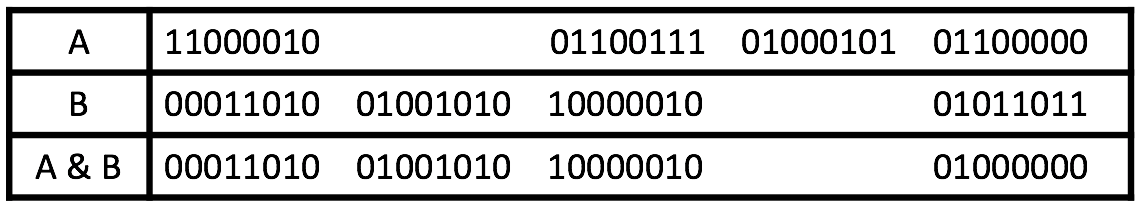
\includegraphics[width=\bigw]{AandB}

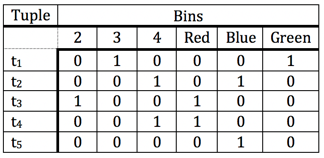
\includegraphics[width=\smallw]{bitmap}

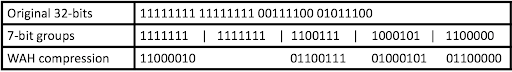
\includegraphics[width=\bigw]{wahcompression}
%
%The motivation for why our research is worth looking at 
%
\section{Introduction}
Data warehouses have become an integral aspect of large-scale computing. Corporations such as Google, Amazon, and Apple use these massive warehouses of servers to store and compute queries on their data. Of course, this computing capability comes at a cost. Not only is conducting operations on such a quantity of servers expensive but, in doing so, those servers develop a large amount of heat. Effects of high server temperatures results in thermal throttling of the CPU's, reducing performance and increasing possibility of hardware failure [Exploring Power-Performance Tradeoffs in Database Systems??].
% Maybe the following link: https://www.anixter.com/content/dam/Suppliers/Upsite/Control%20Data%20Center%20Cooling%20Costs.pdf
Data warehouses, in turn, need to stay cool to allow utilization of their system's full computing capabilities. It can be seen, in fact, that a majority of data warehouses' running costs are due to cooling [Citation hopefully--Exploring Power-Performance Tradeoffs in Database Systems??].
%Would like some feedback on this paragraph and possible citations that are %needed still. -Collin
%Made some editz, hope you like em' booboo :* ~Shane
    %(^^and if you don't like them, then Dr. McClurg made the edits)
There are various ways to combat these limitations; one could be more efficient cooling equipment, however this could result in large upfront costs. Alternatively, software changes could improve load manageability, efficiency, and storage, all while also reducing the thermal impact of large-scale computation.
\par
Software solutions have evolved over the ages, with the main solution being more efficient indexing and storage through the implementation of bitmaps. Bitmaps index data through equality vectors which become cumbersome as the dataset grows.  %I believe there are other means of indexing data beyond just equality vectors, but we can look into this^
Compression of these bitmaps have become a popular strategy to reduce storage space used and performance improvements [Citation about advantages of compression]. Compression of bitmaps have seen many forms as research is done to make the compression and operation more efficient. 
\par 
Compression is useful when the data is immutable but this is not always the case. Updating bitmap indices when data changes without recompiling the whole index would greatly improve efficiency and power consumption. Research has made great strides in updating bitmaps effectively. Our goal was to develop a framework that included updates. 
%
%the background knowledge that will help others to understand some of the paper 
%
\section{Background}
A basic understanding of two concepts is required to sufficiently understand this material; the basics of bitmaps and the basics of Word-Aligned Hybrid (WAH) compression. \par

Bitmaps are two dimensional arrays where the rows represent tuples and the columns represent bins of binary vectors where a “1” represents that the tuple value is at that index location. This enables the ability to conduct fast logical operations on a single column, or group of columns, rather than the entire dataset. For example, one could apply bitmaps to a dataset whose data type contains a number as well as a color. \par

Given the the following dataset, [(3, Green), (4, Blue), (2, Red), (4, Red), (2, Blue)], one could create a bitmap as featured below in Fig. 1. From this bitmap, we can then find all Red values greater than 2 by using an AND of bins 3 and 4 as well as an XAND with the Red bin. \par

%image bitmap.png 

Word-Aligned Hybrid, or WAH, is a popular compression strategy. WAH is often used as the benchmark against which newly created compression strategies are compared. The performance of WAH compression is primarily attributed to the way it processes data as words, or blocks of data whose size correspond with that of the CPU's architecture. An application of WAH in a system using a 64-bit CPU architecture would result in WAH being able to process a word of 64-bits at a time, and so on.
\par 
WAH compression is comprised of two types of words: fills and literals. Data that would constitute a fill would be a consecutive run of a single value, whose length is a multiple of one-bit less than a complete word. Data that would then constitute a literal word would be any combination of 1's and 0's, whose length is also one-bit less than a complete word. For 32-bit words, the fill words would store multiples of 31-bits, and the literals would store 31-bits, whereas in 64-bit words, the fill words would store multiples of 63-bits, and the literals would store 63-bits. 
\par 
In both cases, the remaining bit is used as an identifier, representing whether the compressed word is a fill word or a literal word, denoted as a 1 or 0, respectively. In the case of a literal word in 32-bit architecture, the identifier is set to 0 with the remaining 31-bits following. In the case of fills, the bit immediately following the previously mentioned identifier denotes whether the fill word is of 1’s or 0’s, with the remaining 30-bits represent how many multiples of 31 there are. \par

To show WAH compression we will first show a 128-bit hexadecimal number being compressed into both literal words and a fill word (Fig. 2). We will then feature two 32-bit WAH compressed hexadecimal numbers being AND’ed together (Fig. 3). As you’ll notice A starts out with a run of 1’s. Anything AND’ed against a 1 is just itself so we can just copy over the two first words of B. B than has a fill word that represents two runs of 0’s. As we can recall anything AND’ed with 0 is going to be 0. This means that we can just copy down the fill word into our result. Both of our last words are just literal words that can be AND’ed together without any special case. \par

%image wahcompression.png

%image A&B.png

RoaringBitmap is another popular compression strategy and the second compression algorithm that we compared. Roaring and WAH at their core set out to achieve the same goal. They are meant to compress bitmaps to save space in memory for large datasets. WAH uses RLE (Run-Length Encoding) to achieve this compression while Roaring is a hybrid compression that merges a sorted list and bitmap encoding. \par

%Are we still using RoaringBitmap?? ~Shane

%
%The steps that we took to get where we are
%
\section{Methods}
%
% Maybe talk about how we are setting up a software framework for previous cluster setup. 
% Maybe ease of setup and implementation 
% Features and main uses of our framework
%

Last summer, our team was able to design and build a small scale cluster system that allowed for jobs to be processed using the popular project management tool, Apache Spark. Through this system, we were able to imitate a server system as well as record power measurements along side total energy used. Due to our hardware setup already being constructed, we were able to begin this summer's research focused solely on comparing popular compression techniques and the ability to update such compressed data efficiently and effectively. \par 
%  ^^ This paragraph doesn't really align with our current goals
% --Collin
As mentioned above, we decided to focus ourselves on the evaluation of the popular compression techniques of WAH and RoaringBitMaps. Due to the work that had been done prior, our software had to be based out of Python. This was not a problem initially, as we were able to find open source code on RoaringBitMaps directly from their website that was written in Python. Unfortunately, the same cannot be said for WAH; there was no WAH implementation that was written in Python, therefore developing one was our starting point. \par





%
%What we got out of our research 
%
\section{Results}
<<<<<<< HEAD:Proj2019/Paper/Research Paper.tex
\justify
% Touch again on our main contributions and framework uses
% Possible test results? (Might have to get done later)
=======


>>>>>>> c04a00f0a12b0499fe42b35f72dcbfae5521c1bc:Proj2019/Paper/main.tex
%
%what our results mean for the community
%
\section{Discussion}
<<<<<<< HEAD:Proj2019/Paper/Research Paper.tex
\justify
% How could companies use this research?
% What scenarios would a company want to use this research?
    % What companies would want to use this research? 
    % Tradeoffs with other methods?
=======


>>>>>>> c04a00f0a12b0499fe42b35f72dcbfae5521c1bc:Proj2019/Paper/main.tex
%
%what can be done moving forward
%
\section{Conclusion \& Future Works}


%
%who gave us moneys
%
\section{Acknowledgements}


We would like to thank FMUS, as well as The Women’s Giving Circle, for allowing us to financially continue our research as well as grant us with the opportunity to pursue our  academic growth. We would also like to thank Taylor University for allowing us access to their labs and resources. \cite{bbcCompression95} \par

%
%who gave us  knowledges
%
\section{References}


\bibliography{bibliography}
\bibliographystyle{ieeetr}

\end{document}